\section{Deep Learning}
\label{sec:deep_learning}

Deep Learning ist ein Teilbereich des maschinellen Lernens, der auf tiefen neuronalen Netzen basiert und besonders gut für die Verarbeitung großer, 
unstrukturierter Datenmengen wie Texten geeignet ist.
Ein zentrales Element im Bereich des NLP ist dabei die Nutzung von dichten Vektorrepräsentationen von Wörtern (Word Embeddings).
Nachstehend werden solche Word Embeddings und zentrale Deep-Learning-Verfahren vorgestellt.


\subsection{Word Embeddings}
\label{sec:word_embeddings}

Die klassischen Merkmalsextraktionen in Kapitel \ref{sec:merkmalextraktion} eignen sich gut für klassische Machine Learning Modelle, wie
Support Vector Machines oder Logistische Regression.
Im Vergleich zu Word Embeddings erfassen diese aber keine semantischen Beziehungen.
Word Embeddings verstehen die Bedeutung der einzelnen Wörter je nach Word Embedding in Teilen oder im gesamten Kontext \cite{Deshai:2023aa}
und repräsentieren dabei das ursprüngliche Wort in einem neuen Vektorraum, wobei aber die Eigenschaften des Wortes und seine Verbindungen 
zu anderen Wörtern bestmöglich bewahrt werden \cite{Schaer2023}.
Dabei werden mit maschinellen Lerntechniken verschiedene dichte Vektoren mit einer festgelegten Dimension gebildet.
Word Embeddings sind gegenüber zu BOW (Sparse Matrizen) deutlich speicherschonender.

Das Wort „Bank“ zum Beispiel hat in den Sätzen „Ich setze mich auf die Bank.“ und „Ich raube die Bank aus.“ zwei unterschiedliche Bedeutungen. 
Moderne Word Embeddings erkennen diese und erstellen für die zwei Kontexte/Wörter zwei verschiedene Vektoren \cite{skopos2023wordembeddings}.

In Abbildung \ref{fig:bsp_word_embeddings} wird jedes Wort eines Korpus mit 6 Wörtern als dreidimensionaler Vektor dargestellt.
Ziel eines Word Embedding Verfahrens ist hierbei, dass Wörter mit ähnlichen Bedeutungen oder Kontexten ähnliche Vektordarstellungen haben. 
Die Ähnlichkeit der Vektoren „Katze“ und „Hund“ zeigt die semantische Beziehung zueinander. Die Vektoren „glücklich“ und „traurig“ 
hingegen zeigen in entgegengesetzte Richtungen, was auf ihre gegensätzlichen Bedeutungen hinweist \cite{ibm2024wordembeddings}.

\begin{figure}[htbp]
    \begin{center}
        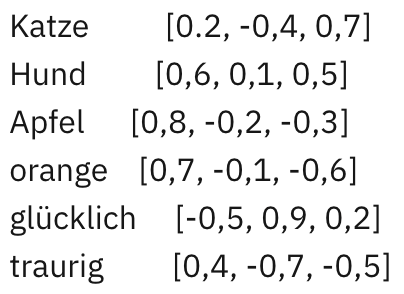
\includegraphics[scale=0.6]{static/bsp_word_embeddings.png}
        \caption{\label{fig:bsp_word_embeddings} Bsp. für Word Embeddings in einem dreidimensionalen Vektorraums \cite{ibm2024wordembeddings}}
    \end{center}
\end{figure}

\subsubsection{Word2Vec}
\label{sec:word2vec}

Das Modell Word2vec verwendet ein neuronales Netzwerk und erfasst numerisch die Ähnlichkeiten zwischen Wörtern aufgrund ihrer 
kontextuellen Merkmale und erstellt darauf aufbauend Embeddings. Am häufigsten wird es zur Analyse der semantischen Verbindungen zwischen Wörtern in einem Textkorpus 
eingesetzt \cite{schumacher2024word2vec}.

Im Beispielsatz 'Mann verhält sich zu Frau wie König zu x.' erkennt Word2vec, dass für $x = \text{Königin}$ gilt. 
Word2Vec löst solche Aufgaben, indem es alle Wörter $x'$ im Gesamtvokabular $V$ ausprobiert 
und das Wort findet, das folgende Gleichung maximiert \cite{CHURCH_2017}:

\begin{equation}
    \hat{x} = \underset{x' \in V}{\operatorname{argmax}} \; \text{sim}(x', \vec{\text{king}} + \vec{\text{woman}} - \vec{\text{man}})
\end{equation}

Wie in Abbildung \ref{fig:cbow_skipgram} zu sehen, gibt es für Word2Vec zwei verschiedene Implementierungen.
Im CBOW-Modell (continuous bag-of-words) wird ein Wort aufgrund seines Kontextes vorhergesagt.
Im Skip-gram-Modell wird hingegen Kontexte aufgrund eines Wortes vorhergesagt.

Bei einem relativ kleines Korpus, empfiehlt Google aufgrund seiner ausgeprägten Fähigkeit mit niedrigfrequenten Wörtern zu arbeiten, 
das Skip-gram-Modell anzuwenden \cite{schumacher2024word2vec}.

\begin{figure}[htbp]
    \begin{center}
        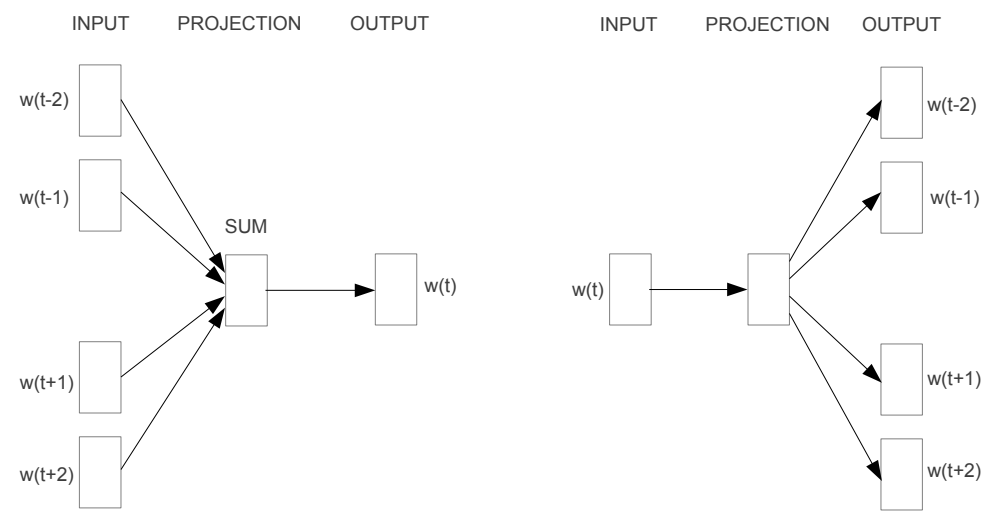
\includegraphics[scale=0.6]{static/cbow_skipgram.png}
        \caption{\label{fig:cbow_skipgram} Vergleich CBOW (links) und Skip-gram (rechts) \cite{mikolov2013}}
    \end{center}
\end{figure}

\subsubsection{GloVe}

Word2Vec fokussiert sich auf Informationen aus lokalen Kontextfenstern, wobei globale Informationen hierbei nicht ausreichend genutzt werden.
GloVe (Global Vectors for Word Representation) verwendet diese globalen Informationen, wodurch semantische Beziehungen zwischen Wörtern erfasst werden.
Wie oft diese zusammen im Korpus vorkommen, wird in einer globalen Co-Occurrence-Matrix zusammengefasst \cite{Wang:2020aa}.

Sei $X$ eine Co-Occurrence-Matrix.
Für jedes Wortpaar $(i, j)$ zeigt $X_{ij}$, wie häufig das Wort $w_j$ im Kontext von $w_i$ erscheint.

Die bedingte Wahrscheinlichkeit, dass Wort $j$ im Kontext von $i$ erscheint, ist:

\begin{equation}
    P(j \mid i) = \frac{X_{ij}}{X_i}
\end{equation}

\begin{figure}[htbp]
    \begin{center}
        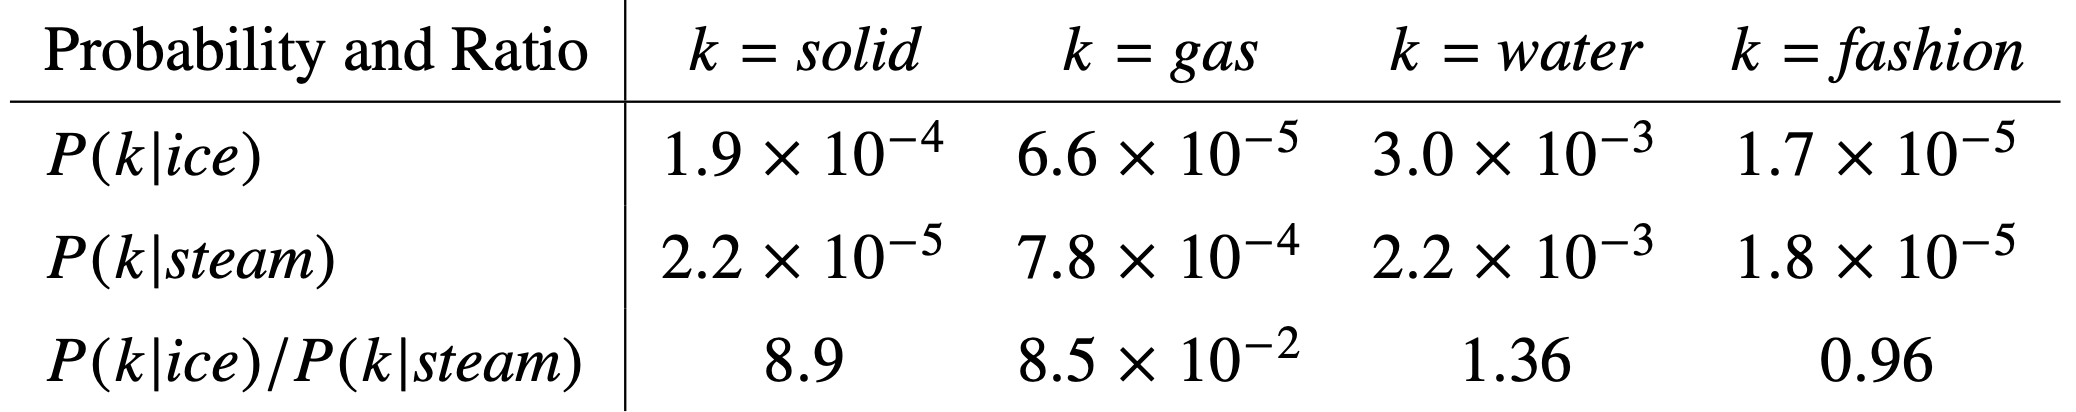
\includegraphics[scale=0.3]{static/glove_matrix.png}
        \caption{\label{fig:glove_matrix} Co-Occurrence-Wahrscheinlichkeiten für die Zielwörter „ice“ und „steam“ mit ausgewählten Kontextwörtern aus einem Korpus mit 6 Milliarden Tokens \cite{pennington2014glove}}
    \end{center}
\end{figure}

Zur Modellierung semantischer Beziehungen vergleicht GloVe Wahrscheinlichkeitsverhältnisse:

\[
\frac{P_{ik}}{P_{jk}} = \frac{X_{ik} / X_i}{X_{jk} / X_j}
\]

In Abbildung \ref{fig:glove_matrix} zu erkennen ist, dass Werte > 1 gut mit Eigenschaften, die spezifisch für „ice“ sind
und Werte < 1 gut mit Eigenschaften, die spezifisch für „steam“ sind korrelieren.
Für $k=solid$ ist der Quotient 8.9. „solid“ hat somit eine größere semantische Beziehung mit „ice“ als mit „steam“.
Für $k=gas$ ist der Wert 0.085. „gas“ passt folglich besser zu „steam“ als zu „ice“.


\subsection{Deep Learning Modelle}
\label{sec:deep_learning_modelle}

Zur Klassifizierung von Nachrichtenartikeln finden unter anderem folgende Deep-Learning-Modelle Anwendung.

\subsubsection{CNN vs. RNN}

Ein Convolutional Neural Network (CNN) ist ein Deep Learning Model (DNN) für Klassifikationsaufgaben,
das Eingabedaten analysiert und dabei unterschiedlichen Merkmalen innerhalb der Daten Gewichtungen zuweist,
um charakteristische Muster zu erkennen und verschiedene Klassen voneinander zu unterscheiden.
Ein großer Vorteil von CNNs ist, dass sie wenig Datenvorverarbeitung benötigen, da sie Rohdaten direkt als Eingabe verarbeiten 
können \cite{aslam2022}.

Ein Recurrent Neural Network (RNN) ist ein DNN zur Verarbeitung sequentieller Daten.
Im Vergleich zu CNNs können sich RNNs an frühere Eingaben erinnern, um aktuelle Vorhersagen zu beeinflussen \cite{Deshai:2023aa}.
Ein RNN nutzt dabei den aktuellen Eingabewert sowie den vorherigen Ausgabewert in jedem Zeitschritt 
und trainiert sich damit selbst, indem es Fehler der Ausgabe zur Eingabe hinzu berechnet.
RNNs eignen sich somit besonders für Probleme in der natürlichen Sprachverarbeitung \cite{Wang:2020aa}, 
da die Reihenfolge der Elemente in diesem Fall entscheidend ist.

Ein zentrales Problem bei RNNs ist jedoch das sogenannte Vanishing Gradient Problem, welches das Lernen 
langer Datenfolgen stark einschränken kann, da lange zurückliegende Eingaben nur noch sehr wenig Einfluss auf das Modell nehmen \cite{aslam2022}.

\subsubsection{LSTM}

Long Short-Term Memory (LSTM) ist ein RNN-Typ im Bereich der Sprachverarbeitung. Das Modell behebt das Problem des 
Vanishing Gradient Problems in klassischen RNNs, indem sie spezielle Speicherzellen verwenden, die Informationen über 
längere Zeiträume hinweg behalten können.
Dadurch sind die LSTM-Modelle effektiv darin, langfristige Abhängigkeiten in sequenziellen Daten zu erfassen und
Beziehungen zwischen Wörtern zu identifizieren \cite{Deshai:2023aa}.

Ein LSTM-Modell besteht aus mehreren Zellen.
Jede dieser Zellen speichert den Zustand des Problems über mehrere Zeitintervalle, während drei Gates den 
Informationsfluss in die Zelle hinein und wieder heraus regulieren.
Das Input-Gate, das Output-Gate und das Forget-Gate \cite{berrajaa2022nlp} (siehe Abbildung \ref{fig:rnnvslstm}).

\begin{figure}[htbp]
    \begin{center}
    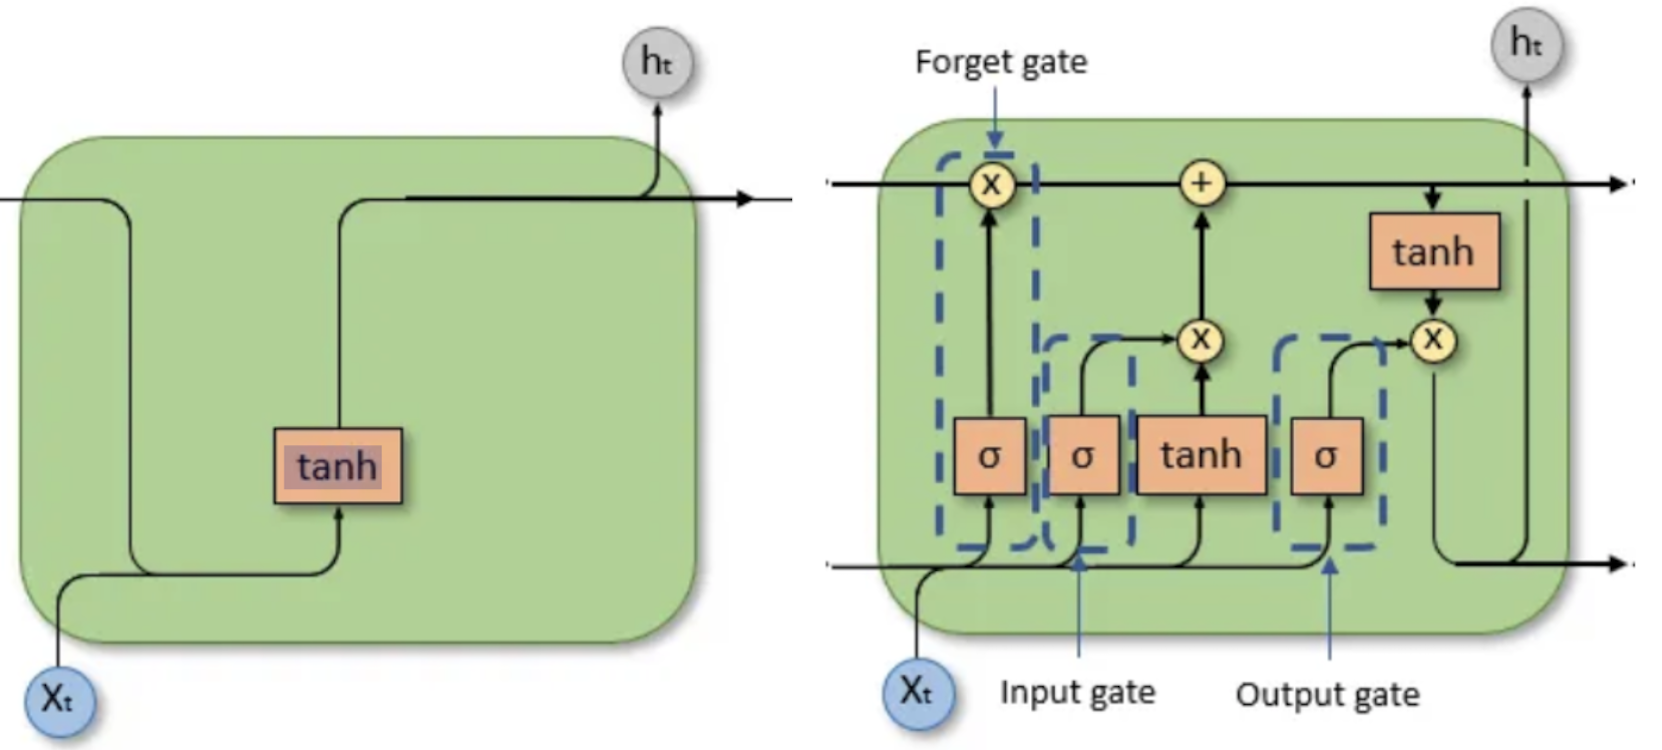
\includegraphics[scale=0.4]{static/RNNvsLSTM.png}
    \caption{\label{fig:rnnvslstm} Vgl. RNN (links) und LSTM (rechts) \cite{aiml2025sequence}}
    \end{center}
\end{figure}

Das Forget-Gate bestimmt, welche Informationen nicht mehr relevant sind und gelöscht werden können. 
Dies hilft, den Speicher der Zelle zu optimieren und unnötige Daten zu entfernen.

Input- und Output-Gate bestimmen, welche neuen Daten hinzugefügt und welche bestehenden 
Daten ausgegeben werden sollen. Sie arbeiten zusammen, um den Informationsfluss zu regulieren.

\subsubsection{BiLSTM}

\begin{figure}[htbp]
    \begin{center}
        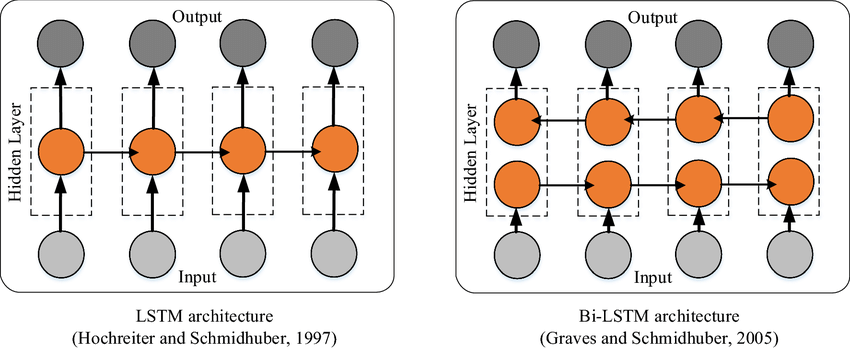
\includegraphics[scale=0.4]{static/lstmvsbilstm.png}
        \caption{\label{fig:lstmvsbilstm} Vgl. LSTM und BiLSTM \cite{shen2021}}
    \end{center}
\end{figure}

Bidirectional-LSTMs (BiLSTMs) sind eine Erweiterung der LSTM-Modelle, bei der zwei LSTMs auf die Eingabedaten angewendet werden. 
In der ersten Runde wird der Input von der ersten LSTM verarbeitet. Anschließend wird der Input in umgekehrter Form auf die zweite LSTM
angewendet (siehe Abbildung \ref{fig:lstmvsbilstm}). Der Input wird somit vor- und rückwärts gelesen, was das Erlernen von 
Langzeitabhängigkeiten verbessert und zu einer höheren Genauigkeit des Modells führt \cite{siaminamini2019}. 

Der Hauptunterschied zwischen Bi-LSTMs und LSTMs besteht daher darin, dass Letztere nur 
Informationen aus der Vergangenheit bewahren, während in Bi-LSTMs durch die Kombination der beiden Leserichtungen sowohl Informationen 
aus der Vergangenheit als auch aus der Zukunft zu jedem Zeitpunkt erhalten bleiben können \cite{shen2021}.